\documentclass[12pt,a4paper]{report}
\usepackage[utf8]{inputenc}
\usepackage[spanish]{babel}
\usepackage{amsmath}
\usepackage{amsfonts}
\usepackage{amssymb}
\usepackage{makeidx}
\usepackage{graphicx}
\usepackage[hidelinks]{hyperref}
\usepackage[left=2cm,right=2cm,top=2cm,bottom=2cm]{geometry}



\begin{document}

\author{Cesar Omar Alvarado Contreras\\
Marco Manzo Torrez\\
Eduardo Robles Vazquez\\
Victor Gabriel Tapia Casillas\\
Fonseca Camaarena Jonathan}

\title{\begin{center}

\includegraphics[scale=1.5]{Escudo.png} 
\end{center}Diseño CAD de un Robot Serial}

\date{
Universidad Politécnica de la Zona Metropolitana de Guadalajara\\
Profesor: Carlos Enrique Morán Garabito\\
19 de septiembre del 2019}

\maketitle
\section{Objetivo:}
Realizar el plano de un robot serial con un software de diseño.
\section{Materiales:}
-Computadora con software (AutoCAD, Inventor, SolidWorks).
-Boceto hecho a mano.

\section{Procedimiento:}
-Basándose en el boceto realizado, se realizó el primer plano del robot serial en AutoCAD, el cual servirá de base para el proyecto anual.
\section{Resultado:}
El resultado de esta práctica es el primer plano del robot serial seleccionado (polar).\\
begin{figure}[h!]
\begin{center}
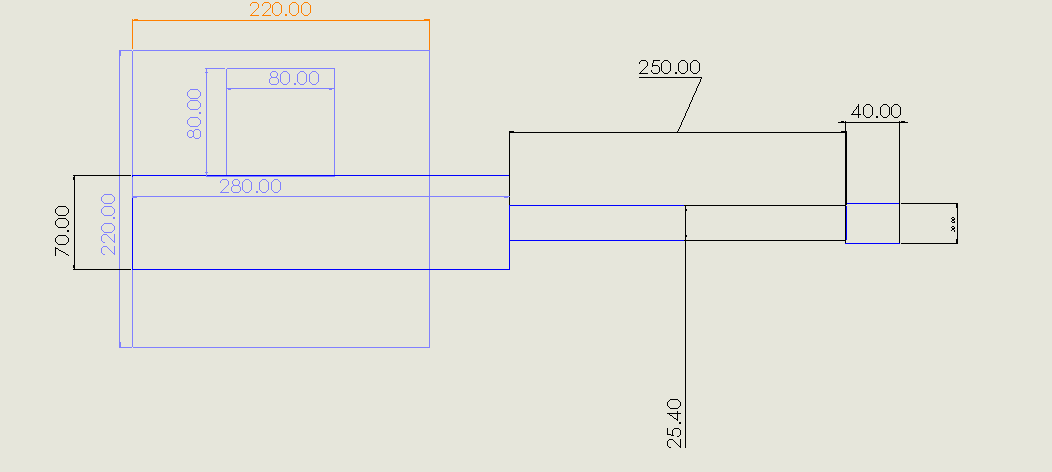
\includegraphics[scale=.6]{DibujoCAD4.png}
Arriba
\end{center}

\begin{center}
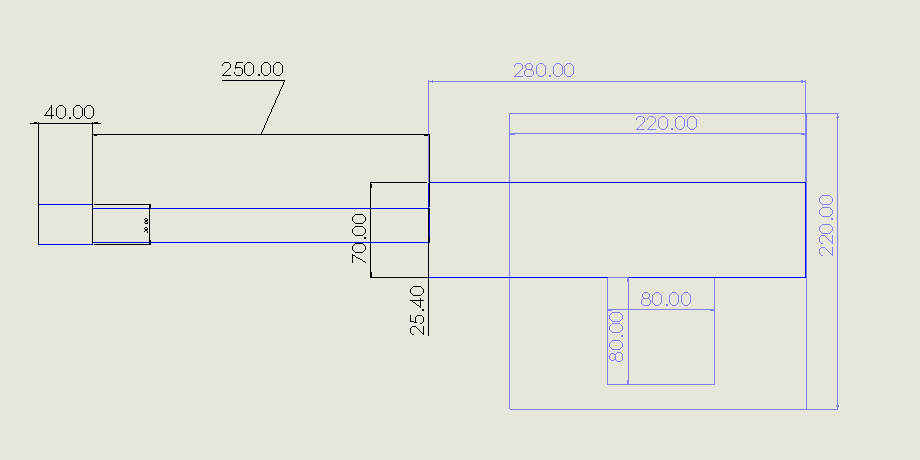
\includegraphics[scale=.6]{DibujoCAD3.png}
Abajo
\end{center}


\begin{center}
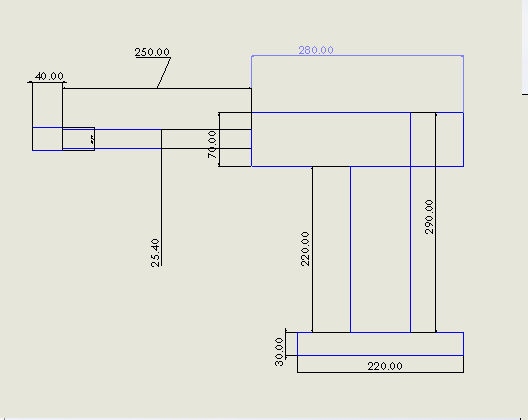
\includegraphics[scale=.6]{DibujoCAD2.png}
Lateral I
\end{center}

\begin{center}
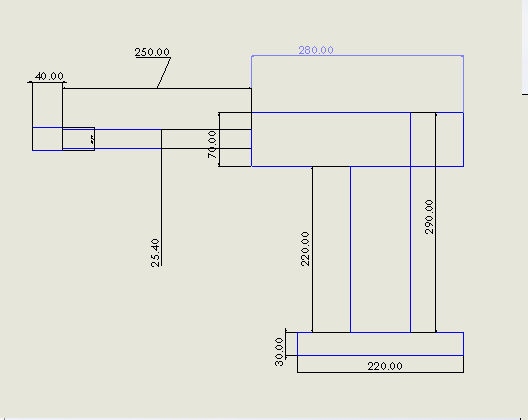
\includegraphics[scale=.6]{DibujoCAD2.png}
Lateral D
\end{center}

\section{Conclusiones:}
Robles Vázquez Eduardo:
En esta práctica llevamos a cabo el diseño CAD de nuestro robot polar, cosa que sirvió de apoyo para el progreso de nuestro proyecto anual/cuatrimestral. El primer paso que realizamos en esta práctica fue hacer un boceto con base a información que teníamos de los robots polares, una vez que el boceto estaba proseguimos a realizar el diseño.\\

Víctor Gabriel Tapia Casillas: Apredimos a utilizar distintas herramientas para el desarrollo de planos de nuestro robot polar.\\

Marcos Manzo Torres:Realizar la construcción de un robot polar desde cero, nos abre un campo de construcción que va desde la selección de materiales y el análisis de fuerzas que actuarán sobre el mismo hasta el diseño final y funcionamiento adecuado. Con el conocimiento previo de la carrera así como las materias que están por venir, debemos realizar las aplicaciones pertinentes de conocimiento, pasar de la teoría a la práctica ca aplicada en un producto final que complementará todo lo que hasta el momento hemos realizado.\\

Jonathan Fonseca Camarena:Entendí en ésta práctica como parte del proceso metodológico del diseño donde la materialización de la idea puede estar por sobre el objetivo. En la medida que lo diseñamos fui consciente que el objetivo se debe acomodar más al dibujo que las ideas, porque si uno empieza a divagar en el dibujo, puede que al final, perdamos el objetivo principal del robot que vamos a crear, por eso es importante tener bien planteados los objetivos, el tiempo y los recursos antes de realizar el boceto y posterior el dibujo.\\

César Omar Alvarado Contreras: El robot dado a diseñar y llevar a cabo como proyecto este ciclo escolar es algo muy poco usual que se desarrolle por ende se propone completar los objetivos que se plantean en este documento siguiendo una organización sobre los eventos a realizar para cada integrante de este equipo, el boceto diseñado es básico y nos da la idea de cómo estructurar el robot.

\begin{center}
Gracias.
\end{center}


\end{document}